%\documentclass{sig-alternate}
\documentclass{acm_proc_article-sp}

\usepackage[utf8]{inputenc}
\usepackage[hyphens]{url}
\usepackage[pdftex,urlcolor=black,colorlinks=true,linkcolor=black,citecolor=black]{hyperref}
\def\sectionautorefname{Section}
\def\subsectionautorefname{Subsection}
\usepackage{graphicx}
\usepackage{caption}
\usepackage{subcaption}
\usepackage{textcomp}
\usepackage{gensymb}
% todo macro
\usepackage{color}
\newcommand{\todo}[1]{\noindent\textcolor{red}{{\bf \{TODO}: #1{\bf \}}}}

\title{From Freebase to Wikidata: The Great Migration}

\numberofauthors{5}
\author{
\alignauthor
Thomas Pellissier Tanon\titlenote{The author was an intern at Google when the majority of the work was done.}
   \affaddr{Google, San Francisco, USA}\\   
   \email{\mbox{thomas@pellissier-tanon.fr}}
\alignauthor
Denny Vrandečić\\
   \affaddr{Google, San Francisco, USA}\\   
   \email{vrandecic@google.com}
\alignauthor
Sebastian Schaffert\\
   \affaddr{Google, Zurich, Switzerland}\\   
   \email{schaffert@google.com}
\and
\alignauthor
Thomas Steiner\\
   \affaddr{Google, Hamburg, Germany}\\   
   \email{tomac@google.com}
\alignauthor
Lydia Pintscher\\
   \affaddr{Wikimedia, Berlin, Germany}\\   
   \email{mail@pintscher.de}
}
\begin{document}

\maketitle

\begin{abstract}
Collaborative knowledge bases that make their data freely available in a~machine-readable form
are central for the data strategy of many projects and organizations.
One such collaborative knowledge base is Freebase, initially launched by Metaweb in 2007,
who were then acquired by Google in 2010.
Another example is Wikidata, a~collaborative knowledge base developed by
Wikimedia Deutschland since 2012 and operated by the Wikimedia Foundation.
Due to the success of Wikidata, Google decided 2015 to shut down Freebase and
help the community with the transfer of Freebase's content to Wikidata.
In this paper, we describe the ongoing transfer efforts and data mapping challenges,
and provide an analysis of the effort so far.
We have created the \emph{Primary Sources Tool}
that we have released as open source to facilitate the transfer of this dataset,
but also future data migrations.
Throughout the migration, we have gained insights into both Wikidata and Freebase,
and share and discuss detailed statistics on both knowledge bases. 
\end{abstract}

% a~category with the (minimum) three required fields
\category{H.4}{\todo{Hierarchy}}{Miscellaneous}

\terms{\todo{Terms}}

\keywords{\todo{Keywords}}

\section{Introduction}

Moving data between two knowledge bases that do not share a~similar design
is usually a~problematic task and requires the careful mapping between their structures.
In this paper, we describe how we facilitated the migration of
Freebase\footnote{Freebase: \url{https://www.freebase.com}} content to
Wikidata.\footnote{Wikidata: \url{https://www.wikidata.org}}
That migration was no exception to this rule, and had a~number of \emph{structural} challenges.
Even more challenging was the \emph{cultural} difference between the two involved communities.
The Freebase and Wikidata communities have a~very different background,
subtly different goals and understandings of their tasks,
and different requirements regarding their data.
\todo{Expand}

The remainder of this paper is structured as follows.
After an introduction to the two collaborative knowledge bases
Freebase and Wikidata in \autoref{sec:background},
we describe our methodology and the metrics used to measure the migration
in \autoref{sec:challenges-of-the-migration}.
In order to support the migration, we have developed a~set of open source tools
that we present in \autoref{sec:primary-sources-tool}.
We then present the results of the migration
and discuss these statistics in \autoref{sec:statistics-of-the-migration}.
The paper terminates with an outlook at proposed next steps
and a~conclusion in \autoref{sec:future-work-and-conclusion}.

\section{Background}\label{sec:background}

\subsection{Freebase}

Freebase is an open source and
collaborative knowledge base created in 2007 by Metaweb and acquired in 2010 by Google.
It was used as the open core of the Google Knowledge Graph,
and also has many use cases outside of Google.

Due to the success of Wikidata,
it was decided to close Freebase and support the migration of its content to Wikidata.
Freebase relies on the notions of \emph{topics}, \emph{facts}, \emph{types}, and \emph{properties}.
Each Freebase topic has a~stable identifier called \emph{``mid''} (for Metaweb ID),
one or more types, and uses properties from these types in order to provide facts.
For example, the Freebase topic for Barack Obama has the mid \texttt{/m/02mjmr}
and the type \texttt{/government/us\_president} that allows the entity to have
a fact with the property \texttt{/government/us\_president/presidency\_number}
and the literal integer ``44'' as the value.

\begin{figure}[!htbp]
\centering
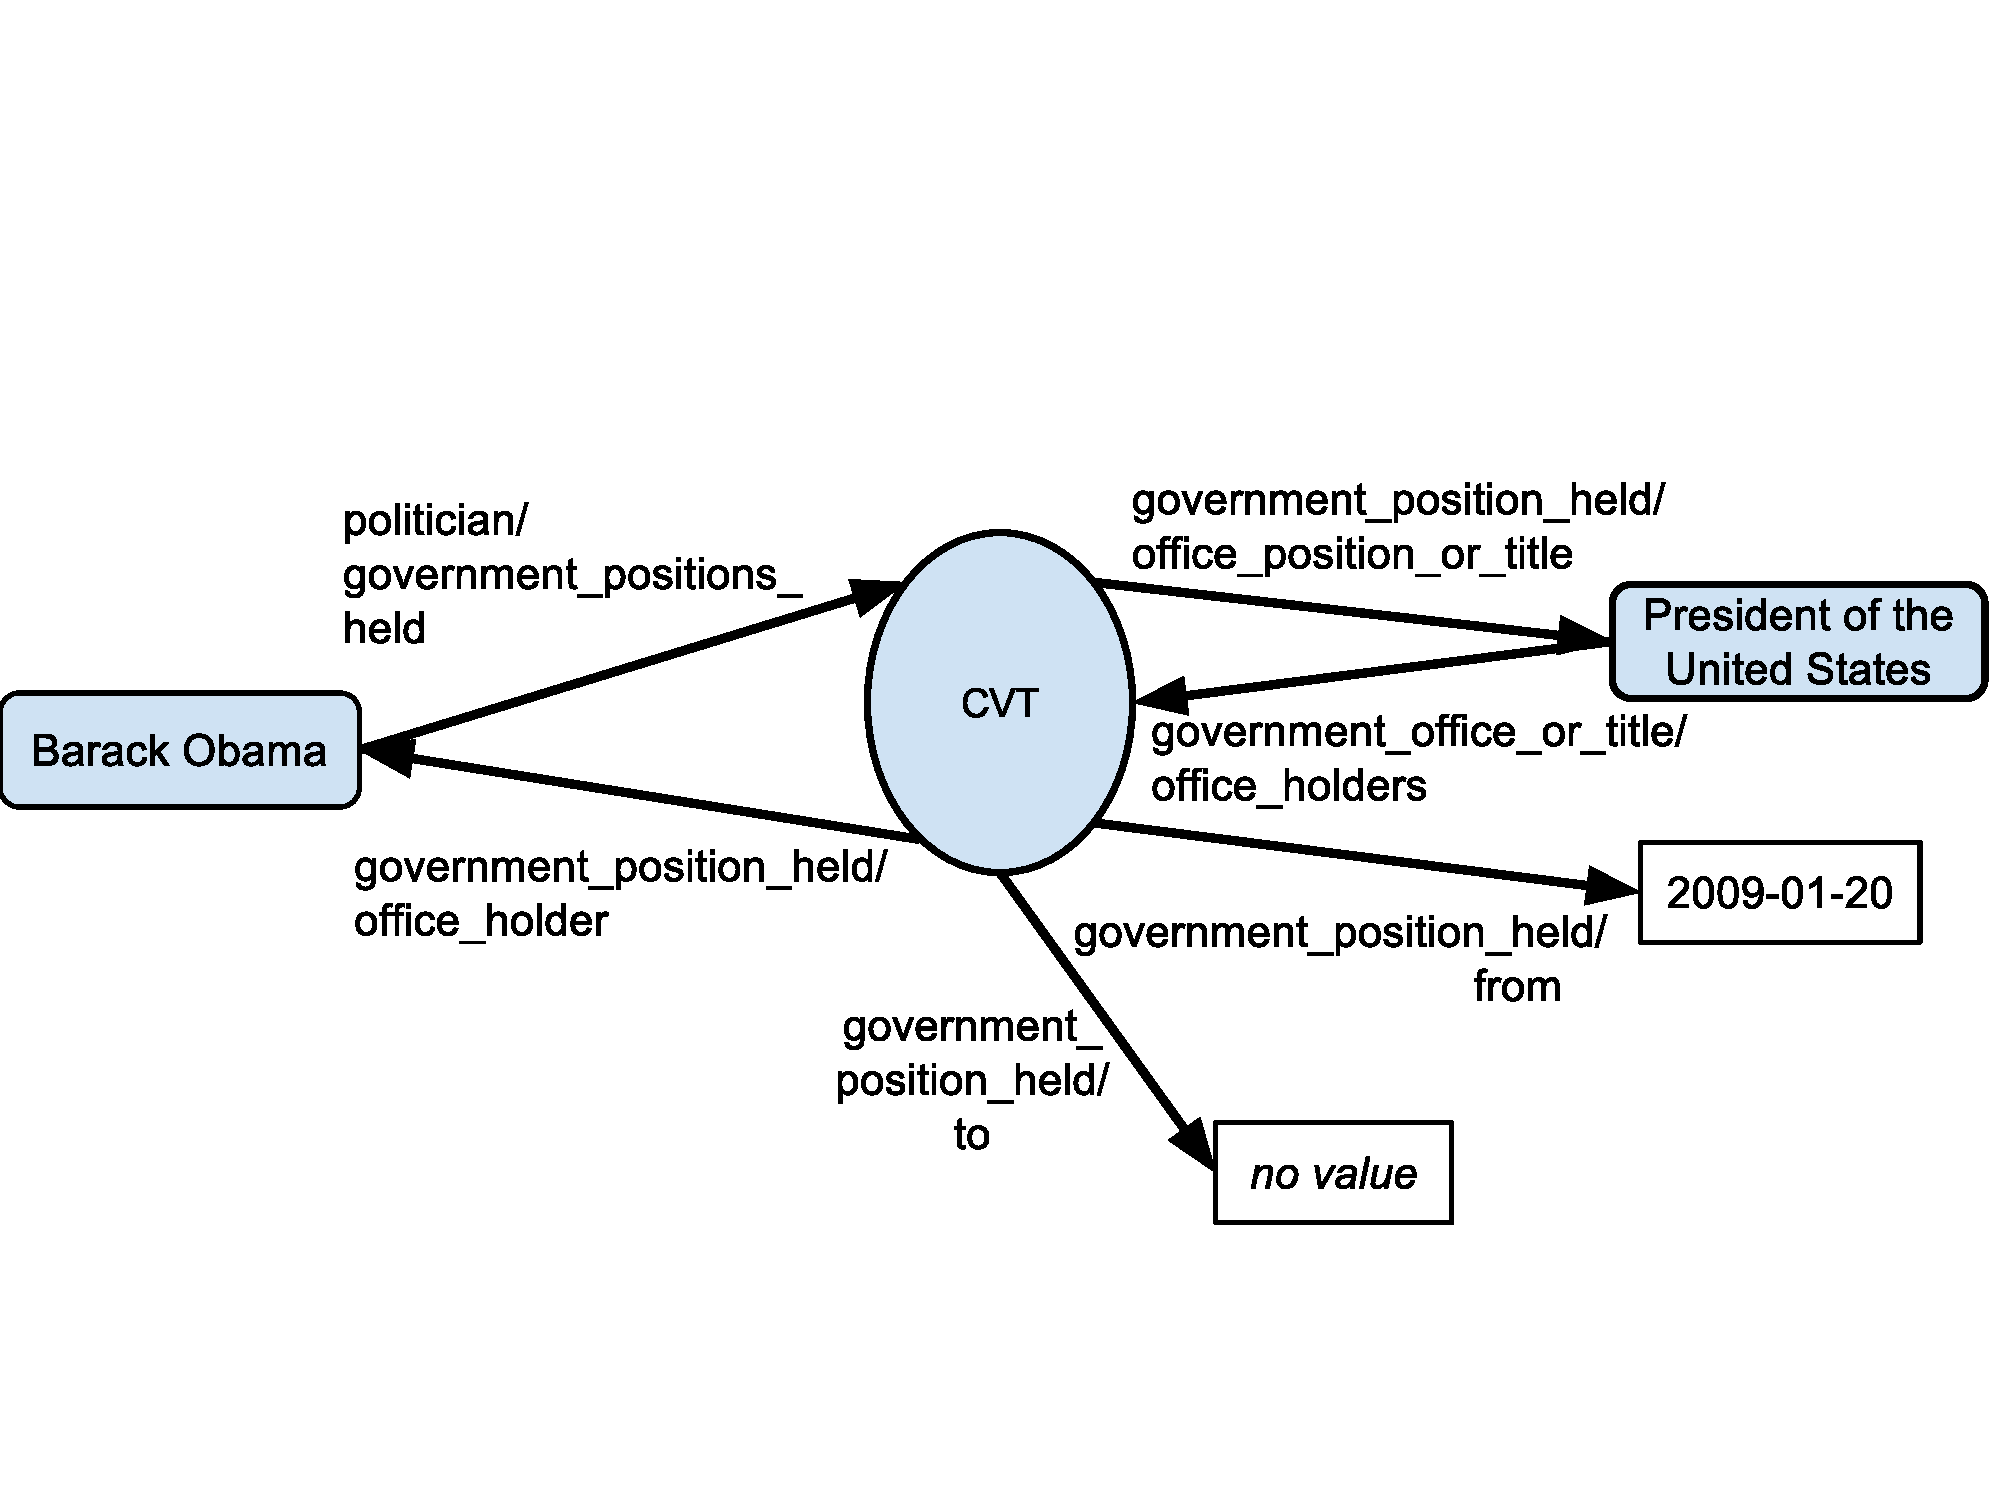
\includegraphics[trim=0cm 3cm 0cm 5cm, width=8.45 cm]{img/freebase-cvt-obama.pdf}
\caption{Exemplary Compound Value Type (CVT) in Freebase: Presidency of Barack Obama.}
%The source is https://docs.google.com/document/d/1ELrBtxxs4ghhe7FloTUnhvpD3f7RFczT7UfxahAfjgE/edit
\label{fig:cvt-obama}
\end{figure}

To represent complex values like geographic coordinates or to annotate relations,
for example, in order to add start and end dates for a~position held,
Freebase has introduced the notion of Compound Value Types (CVTs, see \autoref{fig:cvt-obama}).
They behave like topics, \emph{e.g.}, have a~mid and can have types,
but do not have the \texttt{/common/topic} type.

The content of Freebase has been imported from various sources like Wikipedia
or the Internet Movie Database IMDB,
in consequence Google does not own the copyright of some parts of the content of the knowledge base
like images or long entity descriptions extracted from Wikipedia.
As of the closing of Freebase on March~31, 2015,
it counted more than 3~billion facts about almost 50M~entities.

\subsection{Wikidata}

Wikidata\footnote{Wikidata: \url{https://www.wikidata.org}}
is a~collaborative knowledge base
launched in October 2012 and hosted by the Wikimedia Foundation.
Its community has been growing quickly since the beginning, and as of mid 2015,
the community comprises about 6,000 active contributors.

Wikidata's data model relies on the notions of \emph{item} and \emph{statement}.
An item represent a~concept, has a~stable identifier and may have some labels,
descriptions, and aliases in multiple languages, links to pages about this concept
in the others Wikimedia projects, like Wikipedia, and statements.
Contrary to Freebase, Wikidata encodes with its statements not true facts,
but \emph{claims} from different sources.

A~statement is composed of one claim and zero or more references for this claim.
The claim itself is composed of one main property--value couple that encodes
the main (claimed) fact like ``population is 8,173,900'' and optional qualifiers
to add information about it like ``as of June 2012''.
\autoref{fig:statement} illustrates the used nomenclature with an example.

The content of Wikidata is freely available under a~Creative Commons~0 (CC0) license.
As of mid 2015, Wikidata counted about 66M~statements on 14M~entities.
For more background information about Wikidata, see~\cite{vrandevcic2014wikidata}
by Vrandečić and Krötzsch.
For a~comparison between Freebase and Wikidata,
we refer the reader to~\cite{farbercomparative} by Färber \emph{et~al.}

\begin{figure}[!htbp]
\centering
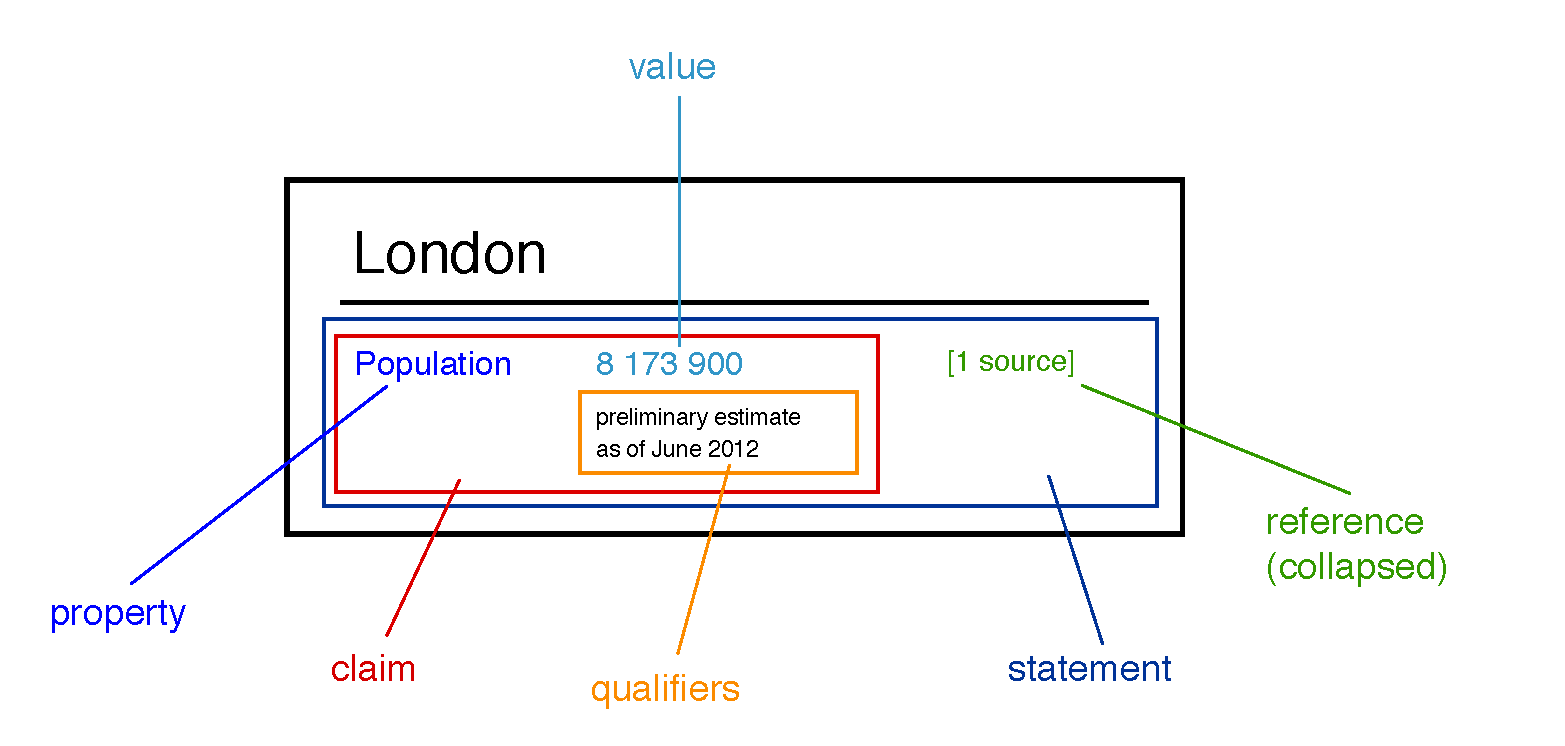
\includegraphics[width=8.45 cm]{img/Wikidata_statement.pdf}
\caption{Wikidata nomenclature illustrated with an example (Source:
	\url{https://commons.wikimedia.org/wiki/File:Wikidata_statement.svg}).}
\label{fig:statement}
\end{figure}

\section{Challenges of the migration}\label{sec:challenges-of-the-migration}

During our ongoing efforts with the migration of Freebase to Wikidata
we were faced with a~number of technical and non-technical challenges
that we will outline in the following.

\subsection{Licensing}
\label{sec:licensing}

The first challenge concerns the licenses under which the datasets are published.
Wikidata is published under a~Creative Commons~0 (CC0~1.0) license
that effectively puts the data in the public domain,
whereas Freebase is published under a~Creative Commons Attribution (CC~BY~2.5) license
and contains data imported from external projects not owned by Google,
like images or descriptions extracted from Wikipedia.
In a~first step, we filtered the Freebase dump for this kind of content
before being able to create a~dump that we could relicense under CC0~1.0.
This step reduced the number of Freebase facts that could be republished by about 42M~facts
from 3~billion facts in the original corpus.

\subsection{References}

The second challenge is that the Wikidata community is very eager to have references
for their statements, \emph{i.e.}, sources that Freebase usually did not store,
except for some specific data like populations and unemployment rates.
For these two specific cases, we have just kept the references from Freebase.
In order to provide the Wikidata community with references for the facts in Freebase,
we have reused data from another Google research project
called Knowledge Vault~\cite{dong2014knowledge} aimed at extracting facts from the Web.
Whereas the fact extraction was usually correct, the pages Knowledge Vault extracted
the references from often do not meet the Wikidata requirements for reliable references:
they include pages in social networks, shopping sites, file sharing hosters, \emph{etc.}
It became necessary to filter the references before potential inclusion in Wikidata
by introducing a~domain blacklist.%
\footnote{URL blacklist:
\url{https://www.wikidata.org/wiki/Wikidata:Primary_sources_tool/URL_blacklist}}

\subsection{Data Quality}
\label{sec:dataquality}

The data quality of Freebase was examined thoroughly by the Wikidata community
and anecdotal evidence indeed confirmed that there were certain challenges.
For example, a~small city in France was assigned an ISO country code,%
\footnote{Freebase item page of the city of Saint-Martin: \url{http://www.freebase.com/m/03cc0d0}}
then Boston (the city in Massachusetts) had the type \texttt{/people/person},
and several other occurrences of data quality issues were revealed.
In consequence, a~fully automatic upload of all the content from Freebase into Wikidata
did not seem advisable as the expectations of the Wikidata community regarding the
quality of automatically uploaded data are high (and rightly so).
Despite the fact that an automated upload of all the data
would have led to accelerated growth in the short term,
such a~fast increase of available data would certainly have endangered
the sense of ownership of the Wikidata community for its data.
As an alternative approach, we decided to rely on crowdsourced human curation
and created the \emph{Primary Sources Tool},
a~software solution that displays Freebase statements
for verification to the user that can be added to the currently shown Wikidata item.
The tool will be described in more detail in \autoref{sec:primary-sources-tool}.

\subsection{Data Topic Mappings}

\subsubsection{Merger of Existing Mappings}

The last challenge concerns the data mappings between Freebase topics and properties
and Wikidata items and properties.
Two mappings between Freebase topics and Wikidata items were initially available,
and in addition to those, we worked on further mappings.
A~first one has been created by Google in October 2013%
\footnote{Freebase mappings: \url{http://developers.google.com/freebase/data}}
and is based on Wikipedia links already present in Freebase: if a~Freebase topic and
a~Wikidata item share at least two Wikipedia links, they are assumed to describe the same subject.
The quality of this mapping is considered very good by the Wikidata community,
who thus have decided to use it and further curate and maintain it by hand.
It maps 1.15M~Freebase topics to their corresponding Wikidata items.
A~second actively maintained mapping has been created by Samsung.%
\footnote{Samsung mappings: \url{http://github.com/Samsung/KnowledgeSharingPlatform}}
It is based on the same idea, but matches a~Freebase topic with a~Wikidata item
even if there is only a~single shared Wikipedia link.
The precision of the mapping is naturally lower compared to Google's mapping,
as there are more wrong matches (often because there is no clear separation between topics
and disambiguation pages in Wikipedia), however, the recall increases to 4.4M~links.
As we have shown in \autoref{sec:dataquality},
that human curation is required before importation anyway,
which is why we have decided to merge the two mapping dumps,
and for the resulting 6,000 conflicts decided to prioritize Google's mapping.

\subsubsection{Reconciliation Based on External Database IDs}

To improve the result, we have also done some reconciliation based on third-party database IDs
shared by Freebase and Wikidata, like MusicBrainz,\footnote{MusicBrainz: \url{https://musicbrainz.org}}
VIAF,\footnote{VIAF: \url{http://viaf.org}} \emph{etc.}
With this technique, we were able to match 800K~external database IDs,
creating an additional mapping for 600K~topics---%
most of them already in the merged version of Google's and Samsung's mappings.
Eventually, this reconciliation effort resulted in an additional 84K mapped items.
We also used Google's Knowledge Graph~\cite{singhal2012} to add 100K~further mappings
by also matching a~topic and an item if they share a~Wikipedia link with the Knowledge Graph item.
There is some potential to add more data by looking at functional relations
like ``father'' and ``mother'', but these relations only apply to relatively small sets of data
(like well known families), and the functional assumptions may run into some edge cases.
For example, the \texttt{/people/person/parents} property in Freebase also covers stepparents,
which may create cases where a~person has more than one male or female \texttt{/people/person/parents}.
Eventually, with these four sources (Google mapping, Samsung mapping, external IDs, Knowledge Graph),
we mapped 4.56M~items in total.

\subsubsection{Mapping Completeness Analysis}

Thanks to these efforts, we have already mapped most of the topics that could be mapped automatically,
which is also backed by the comparably small increases gained from the ID reconciliation approach 
and the Knowledge Graph data described in the previous paragraph.
Furthermore, the \emph{mapped} topics have an average number of facts of about~13.9,
whereas the topics that were \emph{not} mapped have an average number of only 5.7~facts.
We have mapped the majority of topics with more than 47~facts
(191K~non mapped topics \textit{vs.} 195K~mapped topics).
This allows us to conclude that we have mapped the most important items of Freebase.
\autoref{fig:mapped-not-mapped} provides an overview of mapped and non-mapped items
put in relation to the number of facts per item.

\begin{figure}[!htbp]
  \centering
  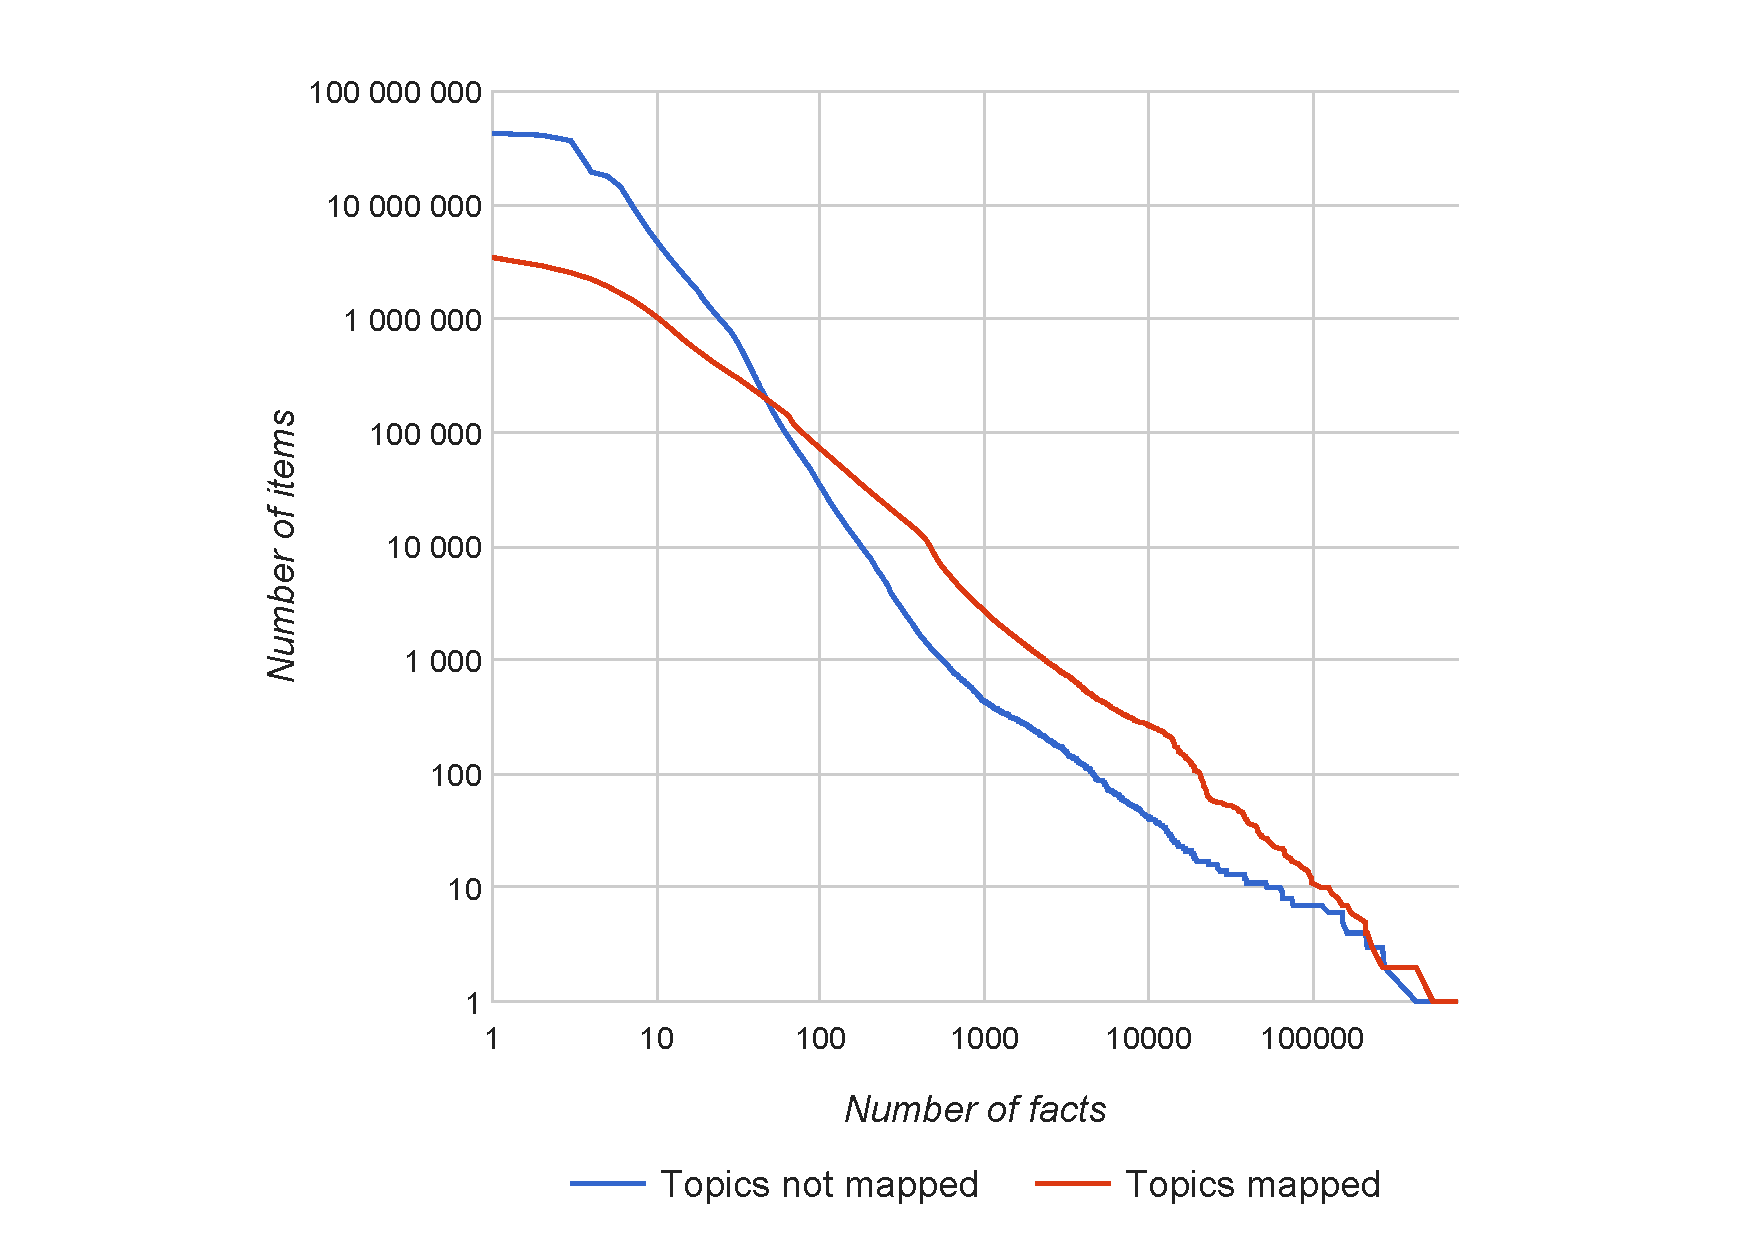
\includegraphics[width=8.45 cm]{img/facts-topics-mapping.pdf}
  \caption{Number of mapped and not mapped topics with more than $x$ facts (log scale on both axes).}
  \label{fig:mapped-not-mapped}
  %Data sheet: https://docs.google.com/spreadsheets/d/1jYGVIqAmyouHKjvhM6FbpgTD8bb5tkJy9PEMELkuMwo/edit  
\end{figure}

\subsection{Data Property Mapping}

For the mapping between Freebase and Wikidata properties we have chosen to do it by hand
with the help of the Wikidata community.
With that, we have been able to quickly map around 360~properties
(note that Wikidata has a~total of 1,660 properties, and Freebase has around 37,700 properties).
For the mapping of properties where the domain are other topics or literals,
this mapping provides the Wikidata property to use.
We have also implemented a~special case for \texttt{/people/person/parents}
in order to be able to map them to Wikidata properties ``father'' and ``mother''
based on the person gender.
The mapping of CVTs (see \autoref{fig:cvt-obama}) is more complicated,
because it is not possible to have a~\mbox{1-to-1} relationship
between Freebase and Wikidata properties: the CVT is linked to the subject topic by one property
and has properties pointing to its component values, whereas the Wikidata statement
has a~main property value group that is qualified by other such groups.
In order to map a~CVT to a~statement, we have to know which of the CVT's properties
should be used as the main value of the statement, with the others being mapped to qualifiers.
In order to keep a~simple mapping that associates one Wikidata property to one Freebase property,
we map both the property that links the topic to the CVT
and the main property of the CVT to the same Wikidata property, and, during the mapping process,
pick the latter as the main property of the CVT.
For example, if we map the CVT shown in \autoref{fig:cvt-obama},
we first use the Wikidata property \texttt{position held (P39)} to map
\texttt{/politician/government\_positions\_held} and
\texttt{/government\_position\_held/office\_position\_or\_title}.
Second, for the qualifiers, we use \texttt{start time (P580)}
for \texttt{/government\_position\_held/from} and \texttt{end time (P582)}
for\linebreak \texttt{/government\_position\_held/to}.
With the resulting property mapping, the created Wikidata statement
looks like the one presented in \autoref{fig:statement-obama}.

\begin{figure}[!htbp]
\centering
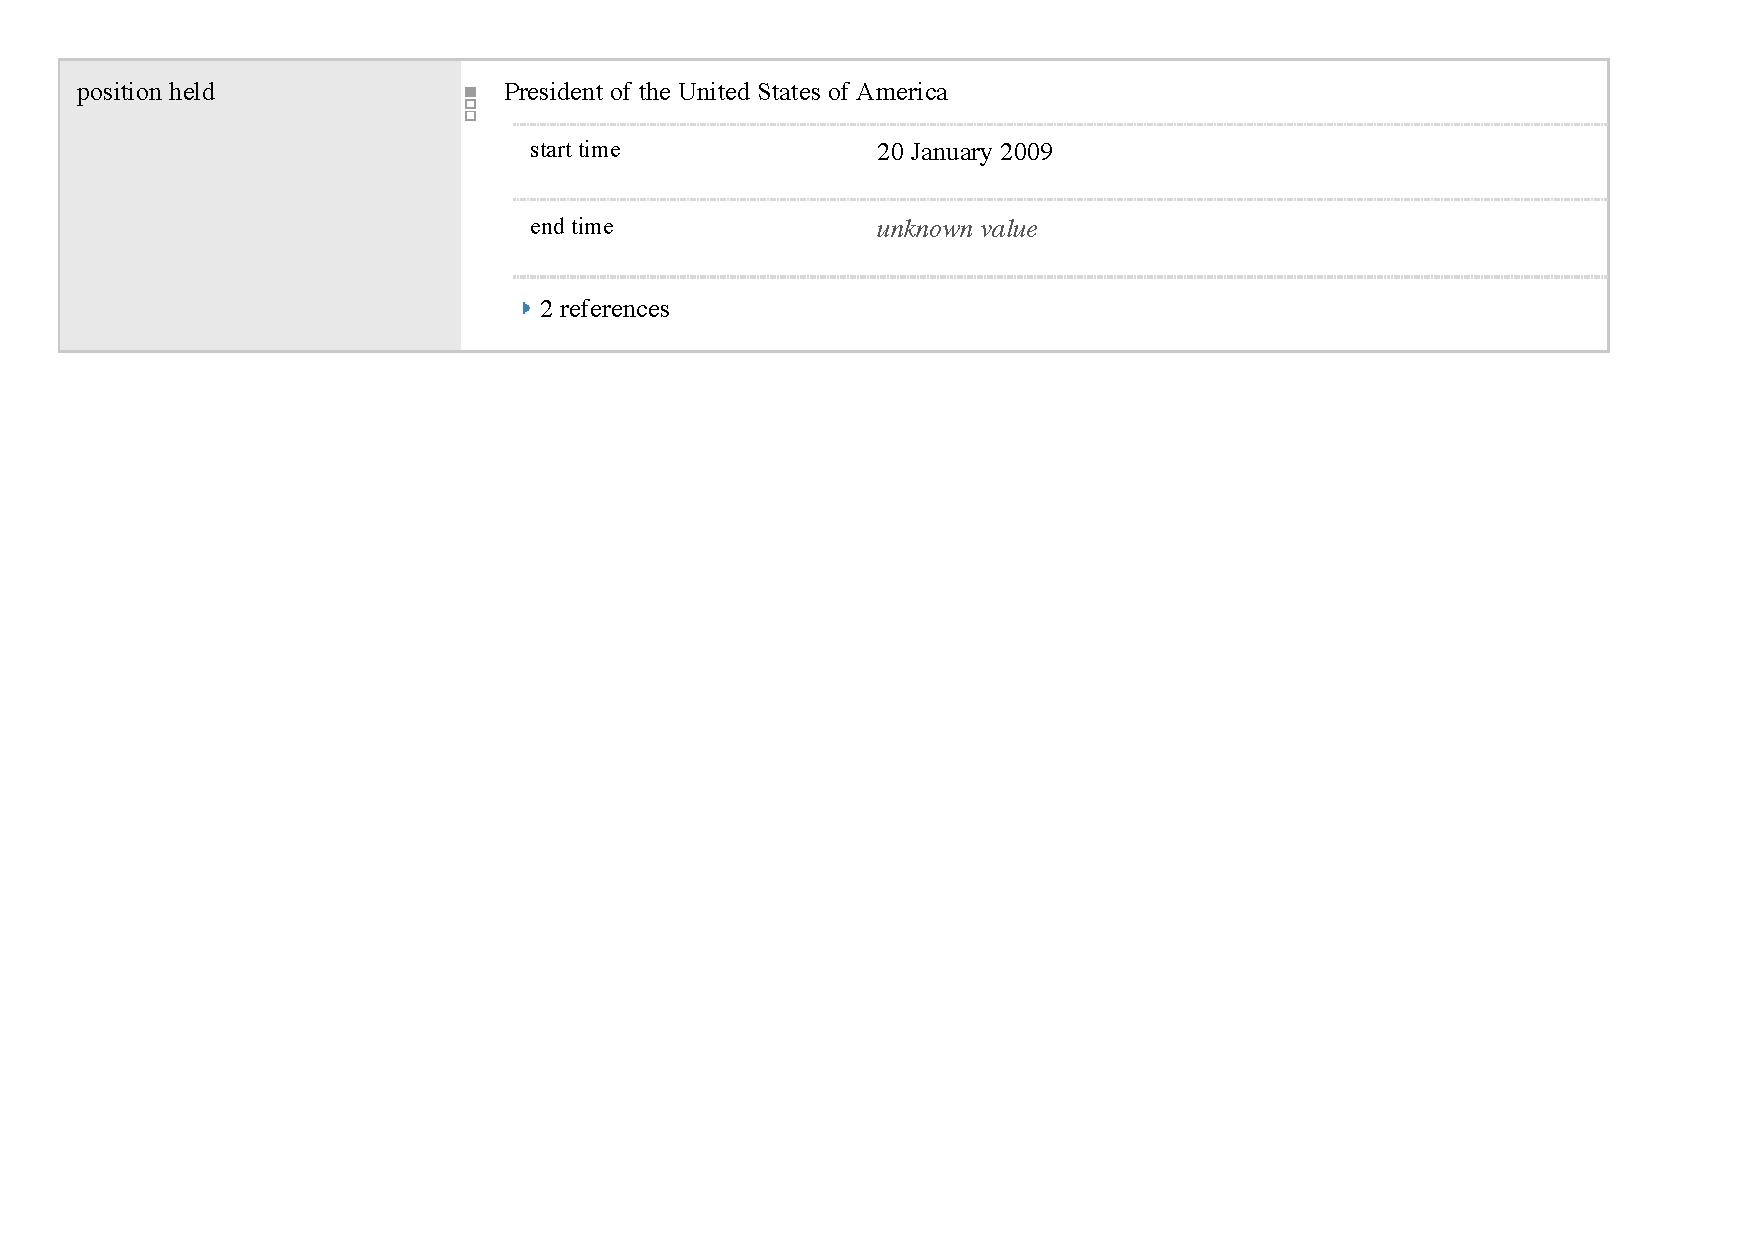
\includegraphics[width=1\columnwidth]{img/wikidata-statement-obama.pdf}
\caption{Wikidata statement for a~Freebase Compound Value Type (CVT).
  See \autoref{fig:cvt-obama} for comparison.}
\label{fig:statement-obama}
\end{figure}

For CVTs that include sources, we map the property that links the CVT
to the source as a~Wikidata reference instead of a~qualifier.
The hardest part then is to actually create the full topic mapping
by considering CVTs and the complex datatypes of Wikidata.
For CVTs, when we have a~triple whose value is a~CVT, we just retrieve it,
map all its component triples (while ignoring ones that cannot be mapped)
and apply the above mechanism to get its main value.
For values, we use the datatype information stored with Wikidata properties
in order to cast values to the right type.
For quantities, we assume that the amounts are precise,
as there is no precision information in Freebase.
For globe coordinates, we have hardcoded the mapping of the \texttt{/location/geocode} CVT
into the globe-coordinate value type of Wikidata
and use the same precision guessing algorithm as the one used by the Wikidata user interface.
For dates, we just map the date and time values (encoded using XSD%
\footnote{\url{ http://www.w3.org/TR/xmlschema11-2/}} types)
to the Wikidata ``time'' datatype, however, filter out dates before 1920 that have
a~higher precision than year because we do not know
if they are relative to the Julian or the Gregorian calendar.
In such cases, we are not able to fill the ``calendar'' value of the Wikidata ``time'' datatype.

\section{Primary Sources Tool}\label{sec:primary-sources-tool}

As outlined earlier, the \emph{Primary Sources Tool} is a~crowdsourced human curation
software solution that displays Freebase statements for verification to the user
so that these statements can be added to the currently shown Wikidata item.
With just one click, the user can reject or approve a~statement,
and, in case of approval, therewith add the statement to Wikidata.
The code of the Primary Sources Tool is openly available
under the terms of the Apache~2.0 license (\url{https://github.com/google/primarysources}).
The tool is deployed as a~so-called gadget,
\emph{i.e.}, as an easily activatable add-on feature in Wikidata.
It is independent from Freebase and can easily be reused to import other datasets into Wikidata.
Therefore, we have implemented an upload API in the back-end
and a~dataset filter in the front-end that allows users
to display only statements from a~selected dataset.
This flexibility is indeed much-wanted, and during the development period of the project
another researcher approached us in order to upload
a~dataset extracted from natural language text.
To visualize the migration progress, we have created a~realtime dashboard
available publicly at \url{https://tools.wmflabs.org/wikidata-primary-sources/status.html}.
At the time of writing (October, 2015), the tool has been used by more than a~hundred users
who performed about 30,000 approval or rejection actions.
More than 12M~statements have been uploaded in total.
\autoref{fig:primary-sources-tool} shows two screenshots
of the tool that integrates nicely with the Wikidata user interface.

\begin{figure}[!t]
    \centering
    \begin{subfigure}[b]{1.0\columnwidth}
        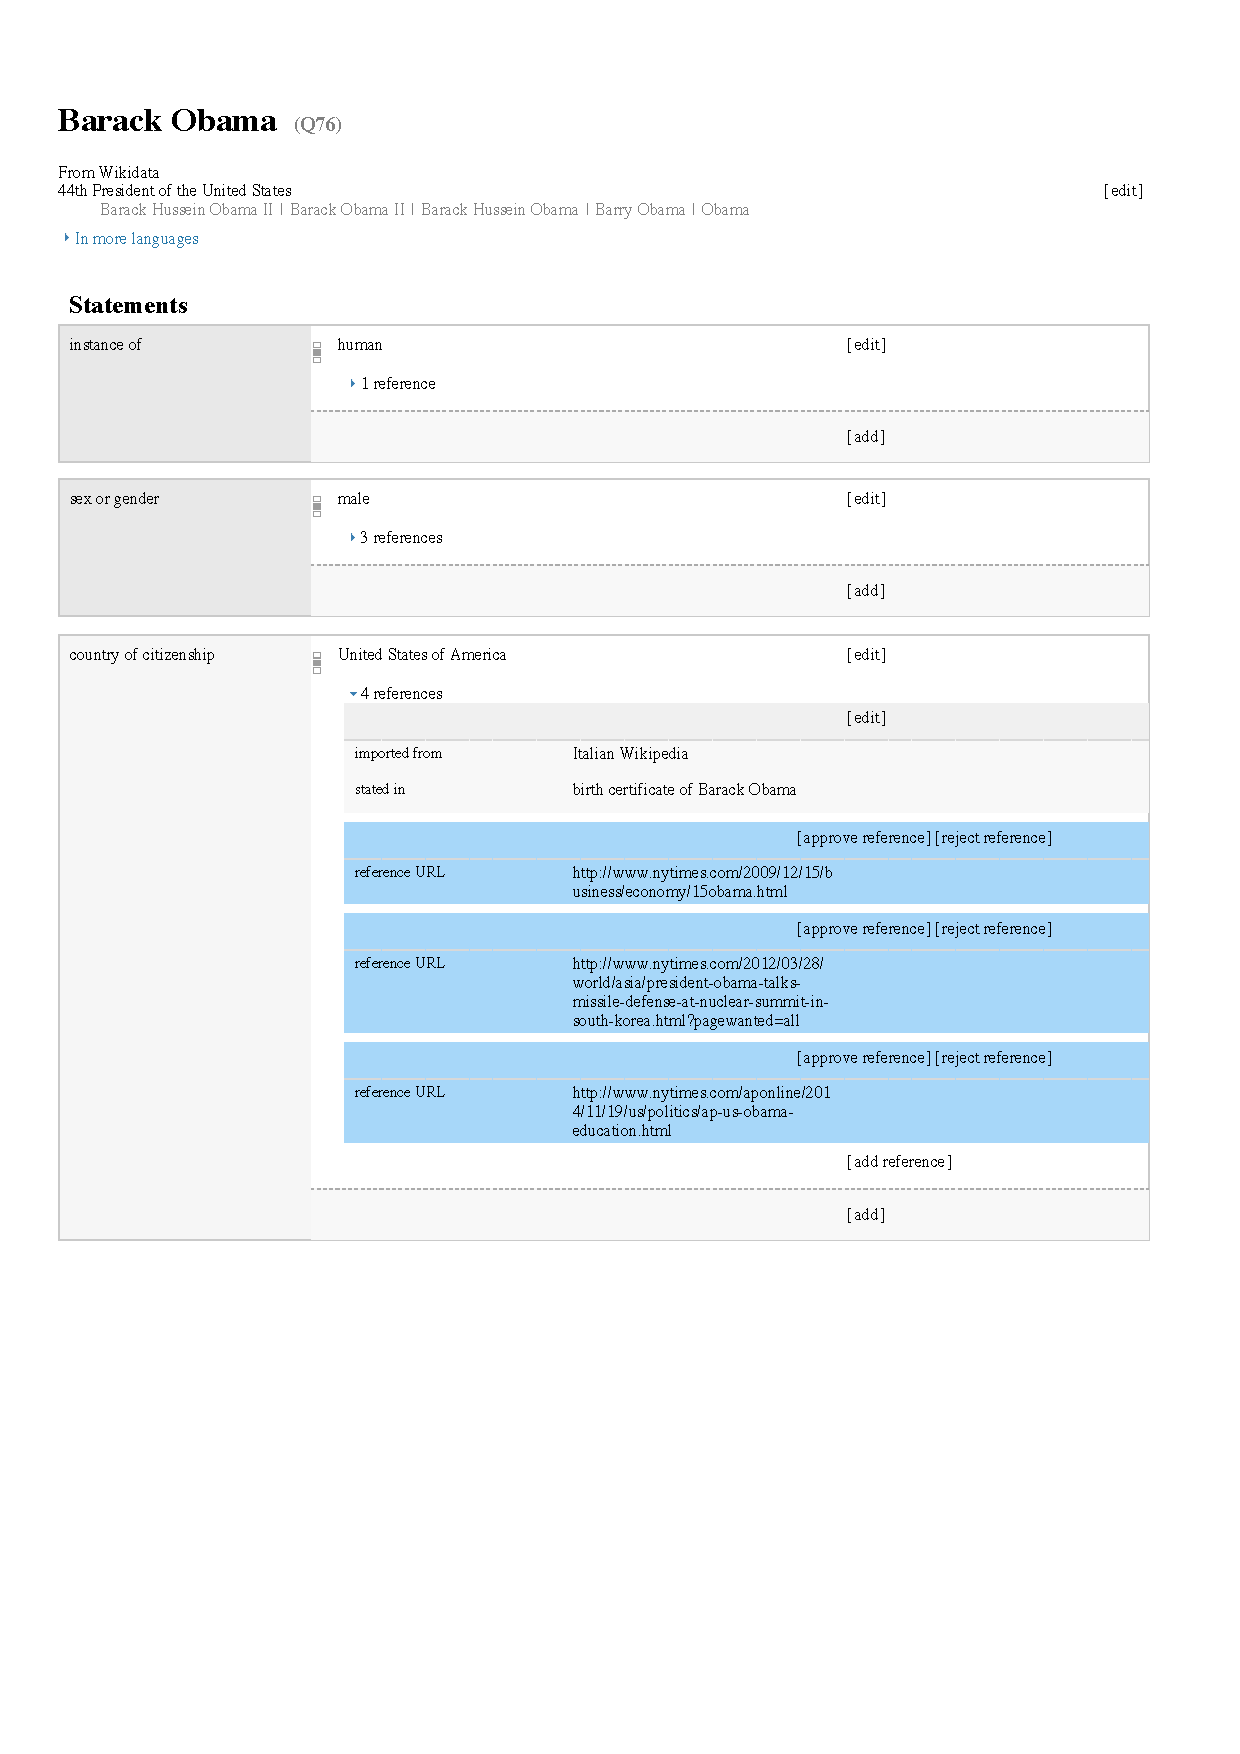
\includegraphics[width=\textwidth]{img/primary-sources.pdf}
        \caption{Incoming references.}
        \label{fig:barack-obama}
    \end{subfigure}
    \begin{subfigure}[b]{1.0\columnwidth}
        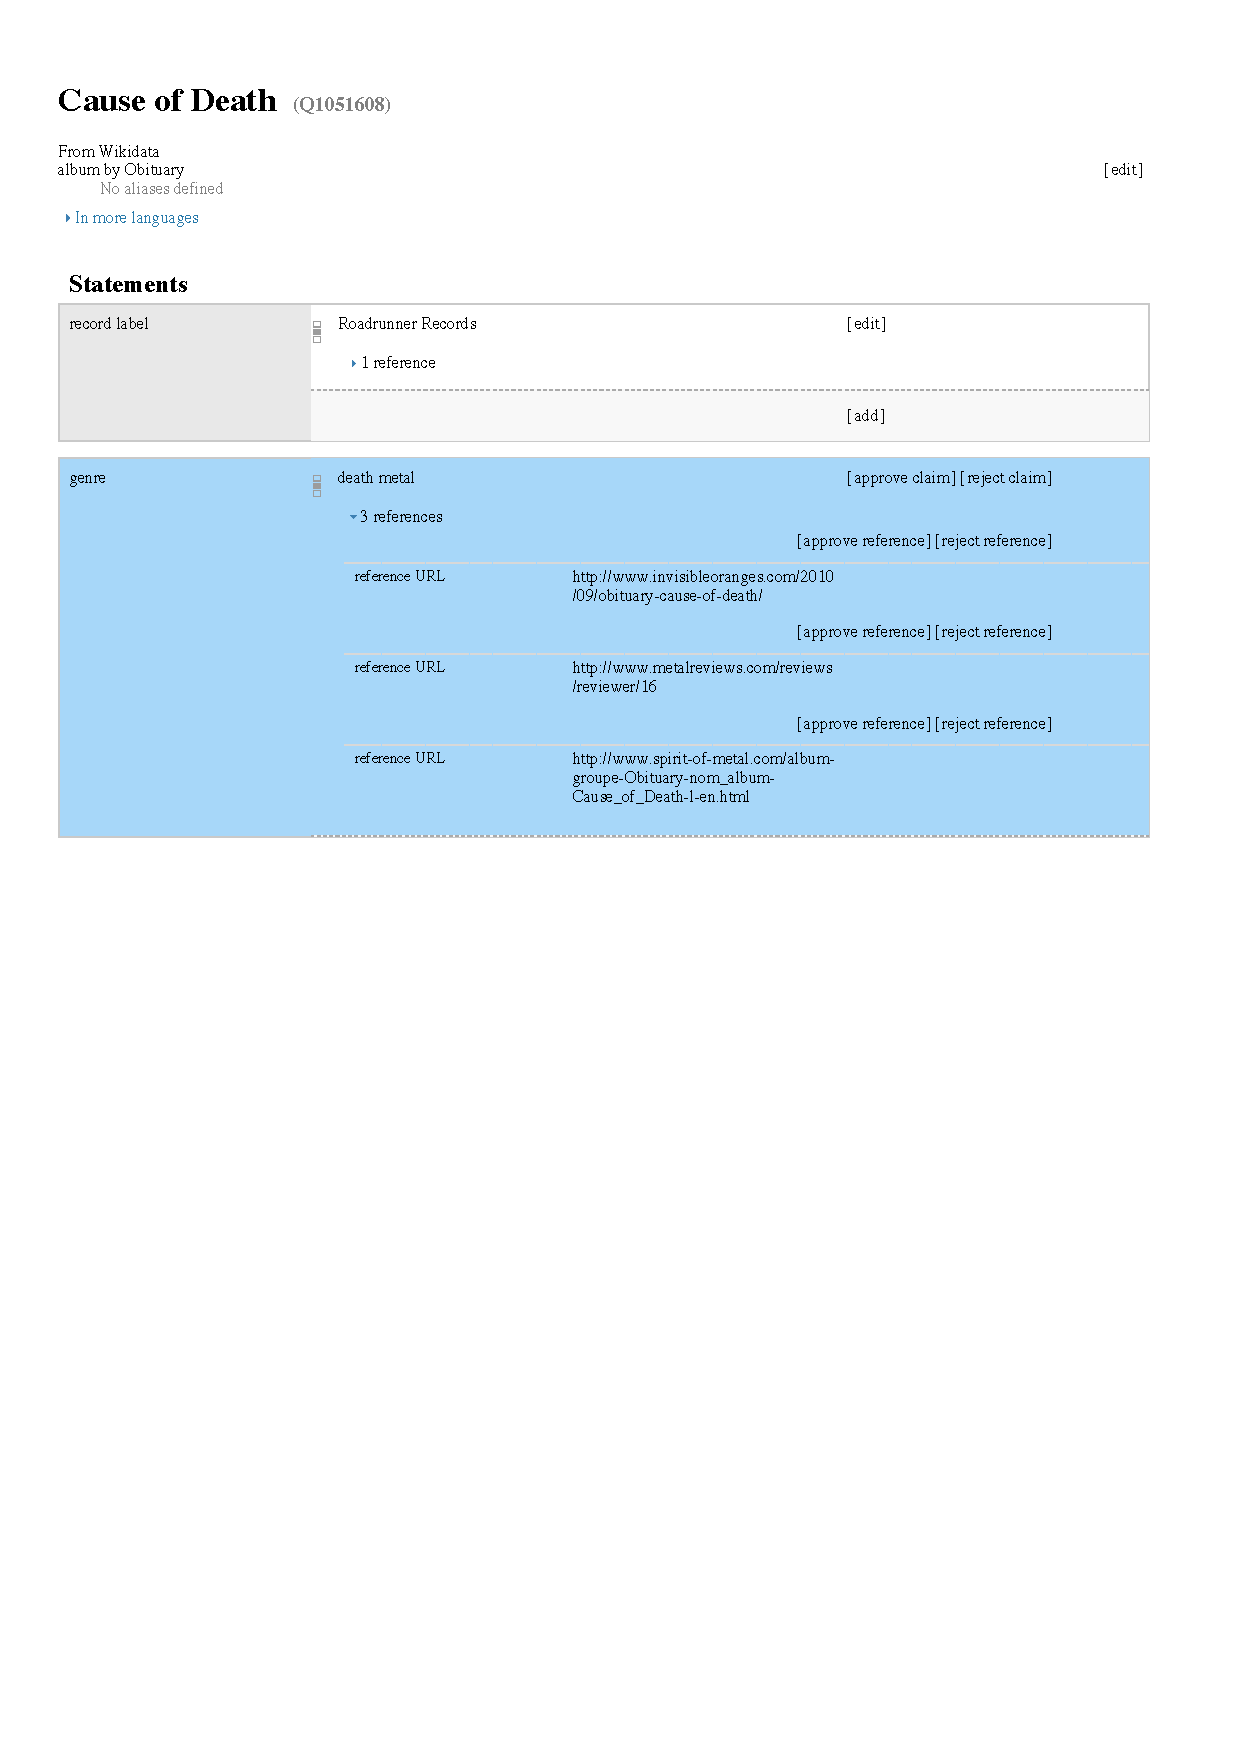
\includegraphics[width=\textwidth]{img/wikidata-cause-of-death.pdf}
        \caption{Incoming claims and references.}
        \label{fig:cause-of-death}
    \end{subfigure}
    \caption{Primary Sources Tool user interface. Statements coming from
       Freebase that are not yet available in Wikidata are shown in light blue.
       Users can approve or reject these statements using the ``approve'' or ``reject'' buttons.}
    \label{fig:primary-sources-tool}
\end{figure}


\subsection{Data Preparation}

In order to prepare the data for integration into the Primary Sources Tool,
we have created a~set of scripts which map the content
of the last Freebase dump to Wikidata statements.%
\footnote{The source code is available under the terms of the Apache~2.0 license:
\url{https://github.com/google/freebase-wikidata-converter}}
The Primary Sources Tool was developed in parallel with the mapping tool.
We first created a~small dataset of around 1M statements
based on few select properties (\emph{e.g.}, \texttt{/people/person/birth\_place})
and deployed both the first dataset and a~basic version of the tool
in order to gather initial user feedback.
In the following, we progressively added more statements to the tool's database back-end.
Thereby, we were able to slowly upscale the tool's database back-end
without risking back-end performance bottlenecks.
The process of adding data in small batches of 1M~to~2M statements per batch
further allowed us to detect some potential issues in the front-end
and fix them before they became actual problems.
Another positive side-effect of this approach was that it allowed us to gather quick feedback
from the community about the already mapped data and thus to adapt the mapping scripts easily
and correct minor issues with the data early on already in the back-end.
Upon approval or rejection of either a~claim or a~reference,
the Wikidata item page in question reloads in order to reflect
the potentially changed state of the migration, as,
in case of incoming claims with references, freshly accepted claims 
can require incoming references to be attached elsewhere in the hierarchy. 

\subsection{Back-end of the Tool}

The objective of the back-end was to have a~REST API allowing us
to serve data efficiently to the front-end of the tool and
providing statistical data about the approvals and rejections done over time.
As the resources of the Wikimedia foundation are limited,
the back-end was implemented in highly optimized C++
and runs as a~FastCGI application in the lighttpd Web server.
\autoref{fig:architecture} shows the overall architecture of the Primary Sources tool.

\begin{figure}[!htbp]
    \centering
    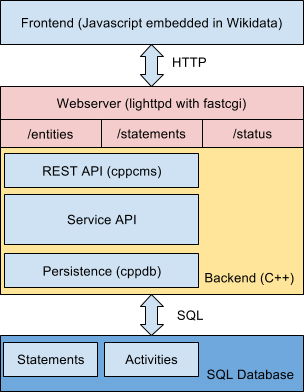
\includegraphics[width=.7\columnwidth]{img/architecture.png}
    \caption{Primary Sources Tool architecture. The front-end is implemented in
      JavaScript and sends HTTP requests to the C++ back-end to retrieve and
      update entities or statements, which are stored in a~relational database.
      \todo{Create PDF version of the diagram, improve consistency of used terms}}
    \label{fig:architecture}
\end{figure}

Entities and statements are stored in a~relational database (MySQL or SQLite)
and follow the Wikidata data structure with an additional status field
to keep track of statements that either already have been approved or rejected,
or not yet visited.
Statements can be grouped in ``datasets'' and ``uploads'' to
distinguish data from different sources.\footnote{At the time of this writing,
the back-end contained five different datasets.}

The REST API of the back-end supports the following main types of requests:

\begin{itemize}
  \setlength\itemsep{0em}
  \item Get an entity (\emph{i.e.}, its statements) by Wikidata QID
  (\emph{e.g.}, \verb|GET /entities/Q2529789|).
  \item Get a~random entity with unapproved (or approved or rejected) statements
  (\verb|/entities/any|).
  \item Get a~statement by database ID (\verb|GET /statements/1|) or get a~list of
  random statements (\verb|GET /statements/any|).
  \item Set a~new state for a~statement \\(\verb|POST /statements/1?state=approved&user=Alice|).
\end{itemize}

All GET requests support an additional \verb|&state={state}| query parameter to filter by state.
This allows Wikidata developers to examine statements
that have already been updated (\emph{e.g.}, ``return 10 random rejected statements'')
for further analysis.
The default of this parameter is \verb|unapproved|.

In addition to these main request types, the REST API also provides endpoints
for importing and deleting datasets, as well as for retrieving the system's status.%
\footnote{The system's status is also presented in more convenient form at
\url{http://tools.wmflabs.org/wikidata-primary-sources/status.html}.}

All update activity around statements is logged in an activity log
for statistical purposes using the Wikidata user name of the user who performed the update.
Activity information can be displayed in an aggregated leader board form
(top users, top rejecters, trends, \emph{etc.}) to add aspects of gamification to the migration process.

\subsection{Front-end of the Tool}

For the front-end, our objective was to make the migration process
as close to the natural Wikidata editing flow as possible.
Ideally, the user should barely notice the different underlying datasources
when navigating Wikidata.
To achieve this, we have in a~first step created a~Wikidata \emph{user script}.
Wikidata user scripts are part of the Wikidata tool chain%
\footnote{Wikidata tool chain:
\url{https://www.wikidata.org/wiki/Wikidata:Tools}}
and are created by users, but unlike gadgets---to be explained in the following---%
do not appear in a~user's preferences.
Instead, one has to add a~line of code into ones \texttt{common.js} file
in order to activate and use the script.
User scripts can be created by anyone and might not always be stable.
Once a~user script has matured, it can be converted into a~\emph{gadget}.
Gadgets are scripts that are likewise created by users,
but which can be simply enabled in user preferences under the section ``Gadgets''.
They can only be edited by administrators and are assumed to be stable.
With our front-end, we went through this maturation steps
and started with a~user script called \texttt{freebase2wikidata.js}%
\footnote{Initial user script:
\url{https://www.wikidata.org/wiki/User:Tomayac/freebase2wikidata.js}}
that we later converted into a~gadget.%
\footnote{Final gadget: \url{https://www.wikidata.org/wiki/MediaWiki:Gadget-PrimarySources.js}}
\autoref{fig:primary-sources-tool} illustrates the user interface in action.
Existing Wikidata statements are shown as usual,
Freebase facts that could potentially be imported into Wikidata are shown in light blue
with instead of an ``edit'' button two new buttons ``approve reference'' and ``reject reference''
(\autoref{fig:barack-obama}) or ``approve claim'' and ``reject claim''
(\autoref{fig:cause-of-death}) respectively.

\section{Statistics on the Migration}\label{sec:statistics-of-the-migration}

\subsection{Quantitative Comparison}

In order to put the statistics in this section in context,
in the following we provide an overview of the size of the last dump of Freebase
from March 2015:

\begin{itemize}
  \setlength\itemsep{0em}
  \item 48M~topics
  \item 2,997M triples
  \item 442M facts owned by Google%
    \footnote{That is, the remaining Freebase triples
      after filtering out data about IDs (\texttt{/type/object/id}),
      types (\texttt{/type/object/type}), labels, descriptions (\texttt{/type/object/name},
      \texttt{/common/topic/description}, \emph{etc.}), and triples removed
      for licensing (see \autoref{sec:licensing})}
  \item 68M~labels
\end{itemize}

As a~direct comparison, below the raw statistics for Wikidata as of August 2015
that make the differences in pure size between the two knowledge bases quite evident.

\begin{itemize}
    \setlength\itemsep{0em}
    \item 14.5M~items
    \item 66M~statements
    \item 82M~labels
\end{itemize}

Why are these numbers so different?
Regarding the number of topics, Freebase has a~lot of topics about subjects
that do not match Wikidata's notability criteria.%
\footnote{Wikidata notability criteria:
\url{https://www.wikidata.org/wiki/Wikidata:Notability}}
For example, Freebase holds data about 11.3M~musical recordings,
8.3M~music canonical versions, 2.6M~ISBNs, \emph{etc.} that are not contained in Wikidata.
We also cannot compare the number of facts and the number of statements directly,
even considering the lower number of topics.
Freebase encodes its knowledge far more redundantly than Wikidata.
To illustrate this, properties in Freebase often have a~\emph{reverse} property
that is used in order to be able to traverse the Freebase graph easily in both directions.
For example, the property \texttt{/people/person/place\_of\_birth} has the corresponding
reverse property \texttt{/location/location/people\_born\_here}
that encodes exactly the same semantic information.
Such reverse properties sometimes exist in Wikidata
(like \texttt{children} for \texttt{father} and \texttt{mother}),
but are far less common.
Another point is that CVTs use a~lot of facts to convey the exact same information
that can be represented with a~single Wikidata statement.
For example, to encode that Barack Obama is the president
of the United States as of June~20, 2009,
Freebase requires more than six facts as shown in \autoref{fig:cvt-obama}.
If we attempted to encode Wikidata statements as if they were Freebase facts, \emph{i.e.},
by removing sources, representing statements with qualifiers using CVTs,
and adding reverse properties, this would lead to 110M facts,
\emph{i.e.}, 167\% of the raw number of statements.
In a~considerable amount of cases, Freebase also contains duplicate data.
For example, many cities in the United States have duplicate CVTs for the population,
where the only change is the encoding of the source.

\subsection{Spatio-Temporal Comparison}

In order to get an idea of the coverage of the two knowledge bases,
we have further created a~spatio-temporal visualization of Freebase and Wikidata 
that is shown in \autoref{fig:time-space}.
The used method is to extract the earliest date and the longitude
linked to each of the entities of the two knowledge bases
and propagate them to the connected entities that do not have such data.
To implement this propagation, we set as value (date or longitude)
the average of the values of the entities whose distance is $<10$
with $2^{-d}$ as weighting, $d$~being the distance between the two entities.
We see that the two knowledge bases follow the same basic patterns,
with their coverage mostly concentrated on Europe and North America.
There are no strong differences between them,
yet coverage of \mbox{\emph{post}-year-2000} entities seems better in Freebase.
Our theory is that this is \emph{(i)}~due to the absence of a~lot of musical data in Wikidata
that in contrast is present in Freebase,
and \emph{(ii)} due to the US population CVTs in Freebase.
The big horizontal lines in \autoref{fig:freebase} and more even in \autoref{fig:wikidata}
can most probably be traced back to places that do not have any linked date,
and in consequence inherit the foundation date of their country.
For Wikidata (\autoref{fig:wikidata}), two lines that are definitely caused by this effect
are the big line over the USA around 1780
and the one covering Russia around 850.
One possible conclusion from this visualization could be that Wikidata,
despite its smaller absolute size, appears to have
a~nearly as complete coverage of the world as Freebase.
Nonetheless, it is very challenging to find objective ways to compare the two databases
and good metrics of success for the migration.
We certainly note that for knowledge bases the amount of triples is not an adequate measure
to judge the proportion of additional good data.

\begin{figure*}[!htbp]
    \centering
    \begin{subfigure}[b]{1.0\columnwidth}
        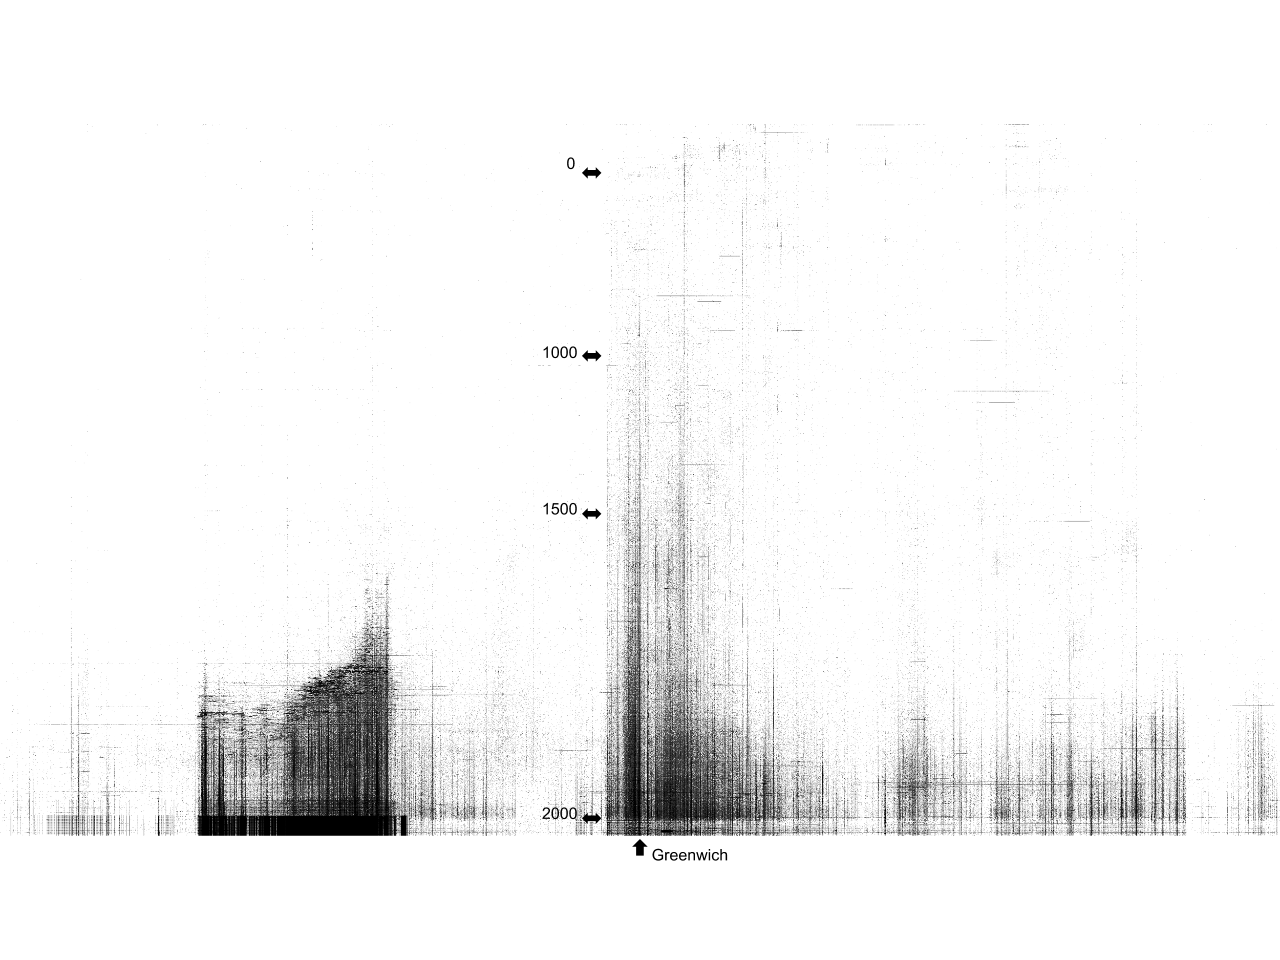
\includegraphics[width=\textwidth]{img/freebase-time-space.png}
        \caption{Spatio-temporal distribution of Freebase.}
        \label{fig:freebase}
    \end{subfigure}
    \begin{subfigure}[b]{1.0\columnwidth}
        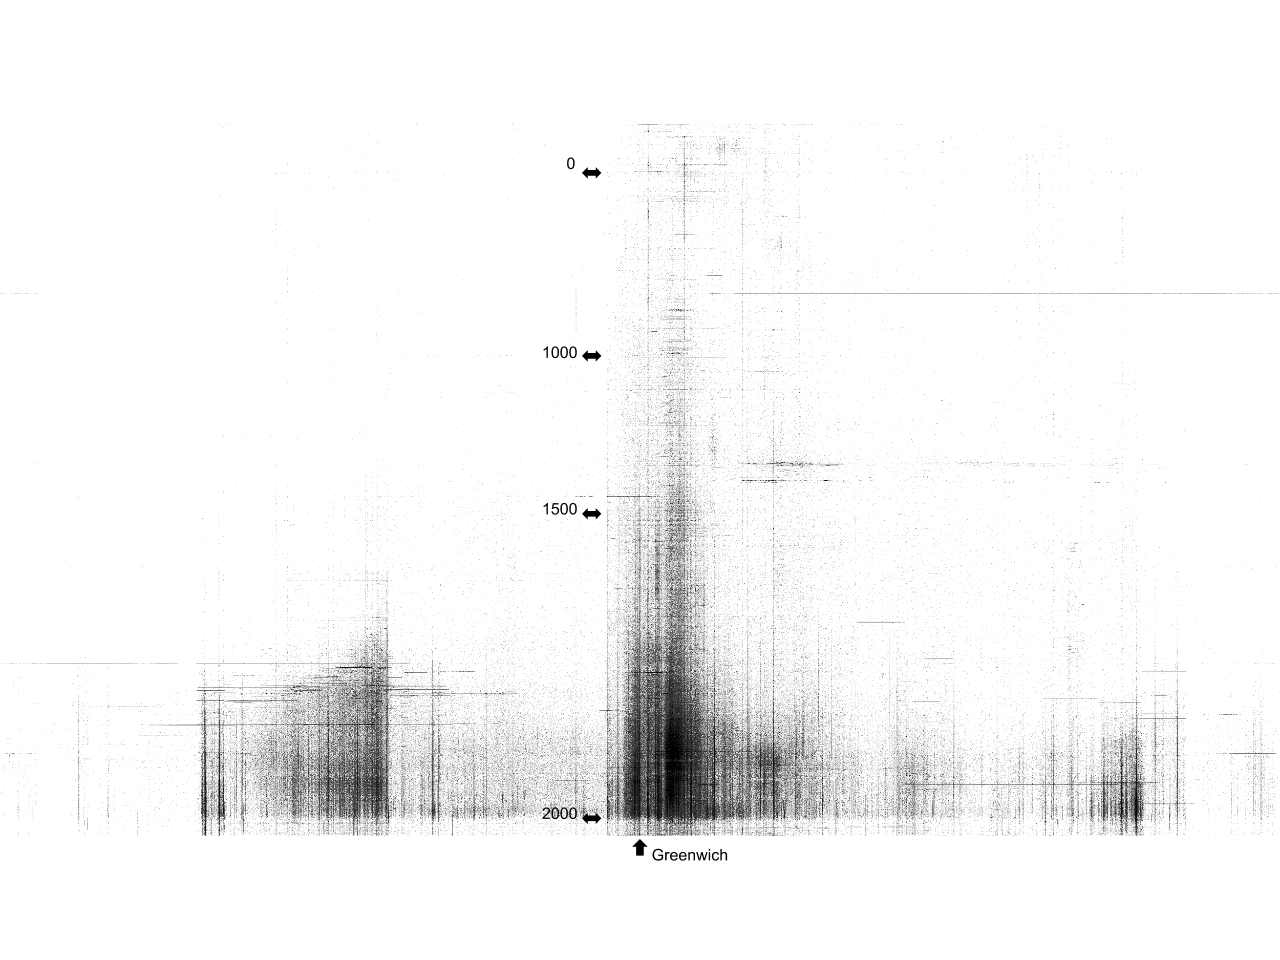
\includegraphics[width=\textwidth]{img/wikidata-time-space.png}
        \caption{Spatio-temporal distribution of Wikidata.}
        \label{fig:wikidata}
    \end{subfigure}
    \caption{Spatio-temporal distribution of Freebase and Wikidata items,
      the $x$ axis shows longitude degrees from 180°~E to 180°~W, the $y$ axis shows time
      from the year 0 to 2015, following a~power law ($y' = y^8$). \todo{Create PDF versions of both diagrams}}
    \label{fig:time-space}
\end{figure*}

\subsection{Raw Statistics}

From the Freebase dump, we have been able to create more than 17M~Wikidata claims
(\emph{i.e.}, statements without references), including 1.5M~IDs.
For that, we have used 31M~Freebase facts.
With additional references, we obtain 19.6M~statements, and, after removing 1M~duplicates
and facts already contained in Wikidata, we obtain 14M~new statements.
Thus, if all these statements were added to Wikidata,
this would lead to a~21\% increase of the number of statements in Wikidata.
The question raises why these numbers are so low compared to the size of Freebase.
We argue that the main reason is that we have only mapped 4.56M~items to Wikidata,
\emph{i.e.}, only 9.5\% of Freebase's topics in total, which are the subject of only 64M~facts.
Even under ideal circumstances, we cannot map more than 64M~statements,
and this is assuming that we could map all reverse properties, which, in fact, we could not.
So leaving aside the not mapped topics, we have created a~statement for more than 24\% of the facts.
If we restrict ourselves to reviewed facts---a~set of 1.6M~human curated facts---we have far better results.
There are 0.58M~facts whose subjects are mapped to Wikidata, and 0.52M~of them
(\emph{i.e.}, 92\%) are converted to Wikidata statements.
58\% of the statements created from reviewed fact are already in Wikidata,
allowing us to add 0.25M~of new reviewed statements to Wikidata.

\section{Future Work and Conclusion}\label{sec:future-work-and-conclusion}

We reckon that the most improvements can be achieved
by extending the migration to more Freebase topics
by suggesting Wikidata users to create new Wikidata items.
A~possible way of realizing this is to create a~user interface%
---possibly leveraging elements of gamification---%
that would allow users to create new Wikidata items for a~suggested topic
or to add a~mapping for them to an existing Wikidata item.
In order to suggest interesting topics to add to Wikidata,
we could rank the not mapped yet topics per number of incoming links
from already mapped topics and filter less interesting types like ISBNs.
Another area for improvement is to upload high quality datasets using a~bot,
like the reviewed facts or some sets for external IDs,
in order to speed up the integration of Freebase content into Wikidata.
We have already started to upload simple reviewed facts about humans
like birth date, death place or gender using a~bot.
We have also begun to import labels that are in Freebase and are absent from Wikidata.
In the 17.2M~Freebase labels for mapped topics, only 0.9M, \emph{i.e.}, 5\%, are missing in Wikidata.

Concluding, in a~fairly short amount of time, we have been able
to provide to the Wikidata community more than\linebreak 14M~new Wikidata statements
using a~novel customizable and generalizable software solution called Primary Sources Tool
that is well integrated into the Wikidata user interface.
The effort needed to map two fairly different knowledge bases has also been a~good occasion
to highlight the difficulty of having good metrics to measure the size
and in consequence the ``value'' of such collaborative knowledge bases.
We envision that this project now with Freebase, and for even more datasets in the future,
will facilitate to increase the completeness of Wikidata.

\bibliographystyle{abbrv}
\bibliography{biblio}

\balancecolumns
\end{document}
